%%%
%
% $Autor: Wings $
% $Datum: 2021-05-14 $
% $Pfad: GitLab/MLEdgeComputer $
% $Dateiname: CAMimx477
% $Version:  $
%
% !TeX spellcheck = de_GB
%
%%%

\chapter{Arducam IMX477}

Für Jetson IMX477 HQ Camera Board, 12.3MP Camera Board für Nvidia Jetson Nano/Xavier NX, Raspberry Pi Compute Module


Farbe: IMX477 Kamera Board für Jetsons

Ein Can't-Miss Update auf IMX219 – Viel bessere Bildqualität und Flexibilität der Linse, dank 53\% mehr Pixel, 92 \% größere Pixelgröße, 192 \% größerer Bildbereich und einer CS-Mount. Maximale Standbildauflösung bei $4056 \times 3040$, Bildfrequenzen: 30 fps \@ Full 12,3 MP, 60 fps \@ 1080P.

Beschleunigt durch Jetson Hardware ISP Engine – unterstützt NVIDIA Argus Kamera-Plugin für H264-Kodierung, JPEG-Snapshots sowie Gain, Belichtung, Framerate und Gruppe, Hold-Kontrolle.

4-Lane Camera for the Future - Route out all 4 data spurs to the camera connector for customized Carrier boards with 4-spane CSI-Anschluss and future 4-spane camera driver updates. For the new version (R32 4.4), please go to the link:

\url{https://github.com/ArduCAM/MIPI_Camera/releases} 

Hinweis:

\begin{itemize}
  \item C/CS-Objektiv ist nicht im Lieferumfang enthalten. 
  \item Raspberry Pi 2/3/4/Zero funktionieren nicht damit. Nur die Computer-Module tun. 
  \item Der Kameratreiber muss installiert werden:
  
       \url{https://github.com/ArduCAM/MIPI_Camera/Releases/Tag/v0.0.2}; 
       
       Für die neue Version (R32 4.4) gehen Sie bitte zu dem Link: \url{https://github.com/ArduCAM/MIPI_Camera/releases}
  \item  Es kann auch auf dem Raspberry Pi Compute Modul verwendet werden. (wie CM3, CM3+), aber nicht kompatibel mit Standard Raspberry Pi Modellen
\end{itemize}


\begin{figure}
    \begin{center}
        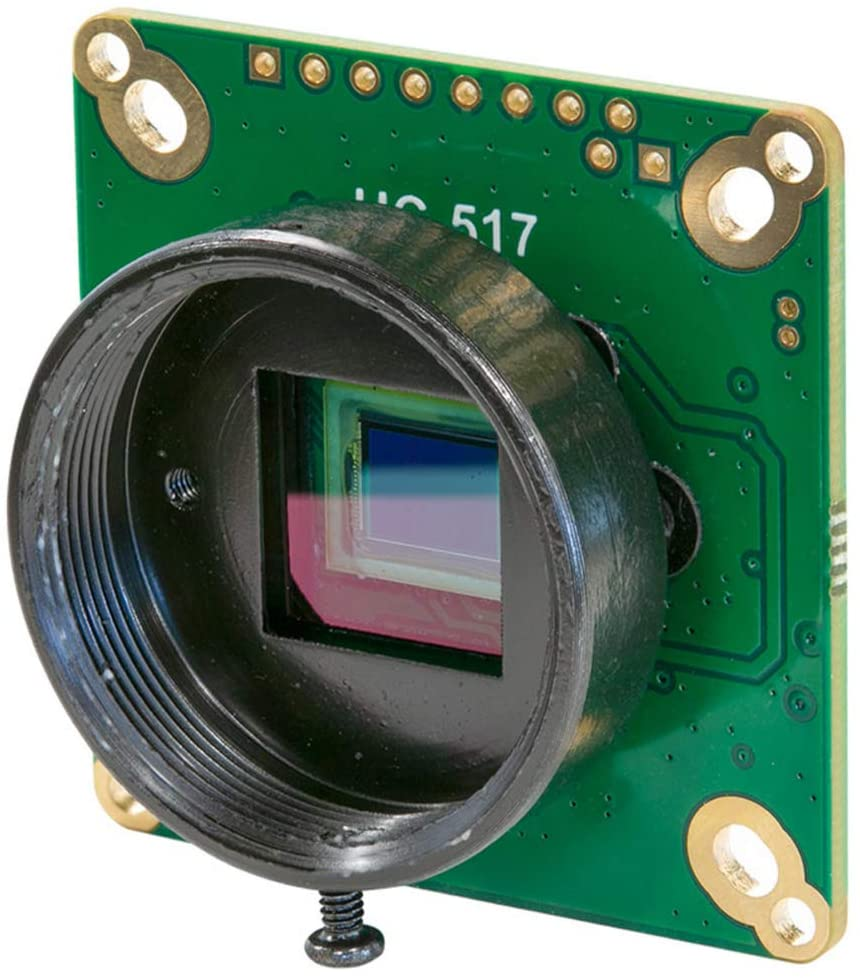
\includegraphics[scale=0.15]{CAM/imx477/imx477}
        \quad 
        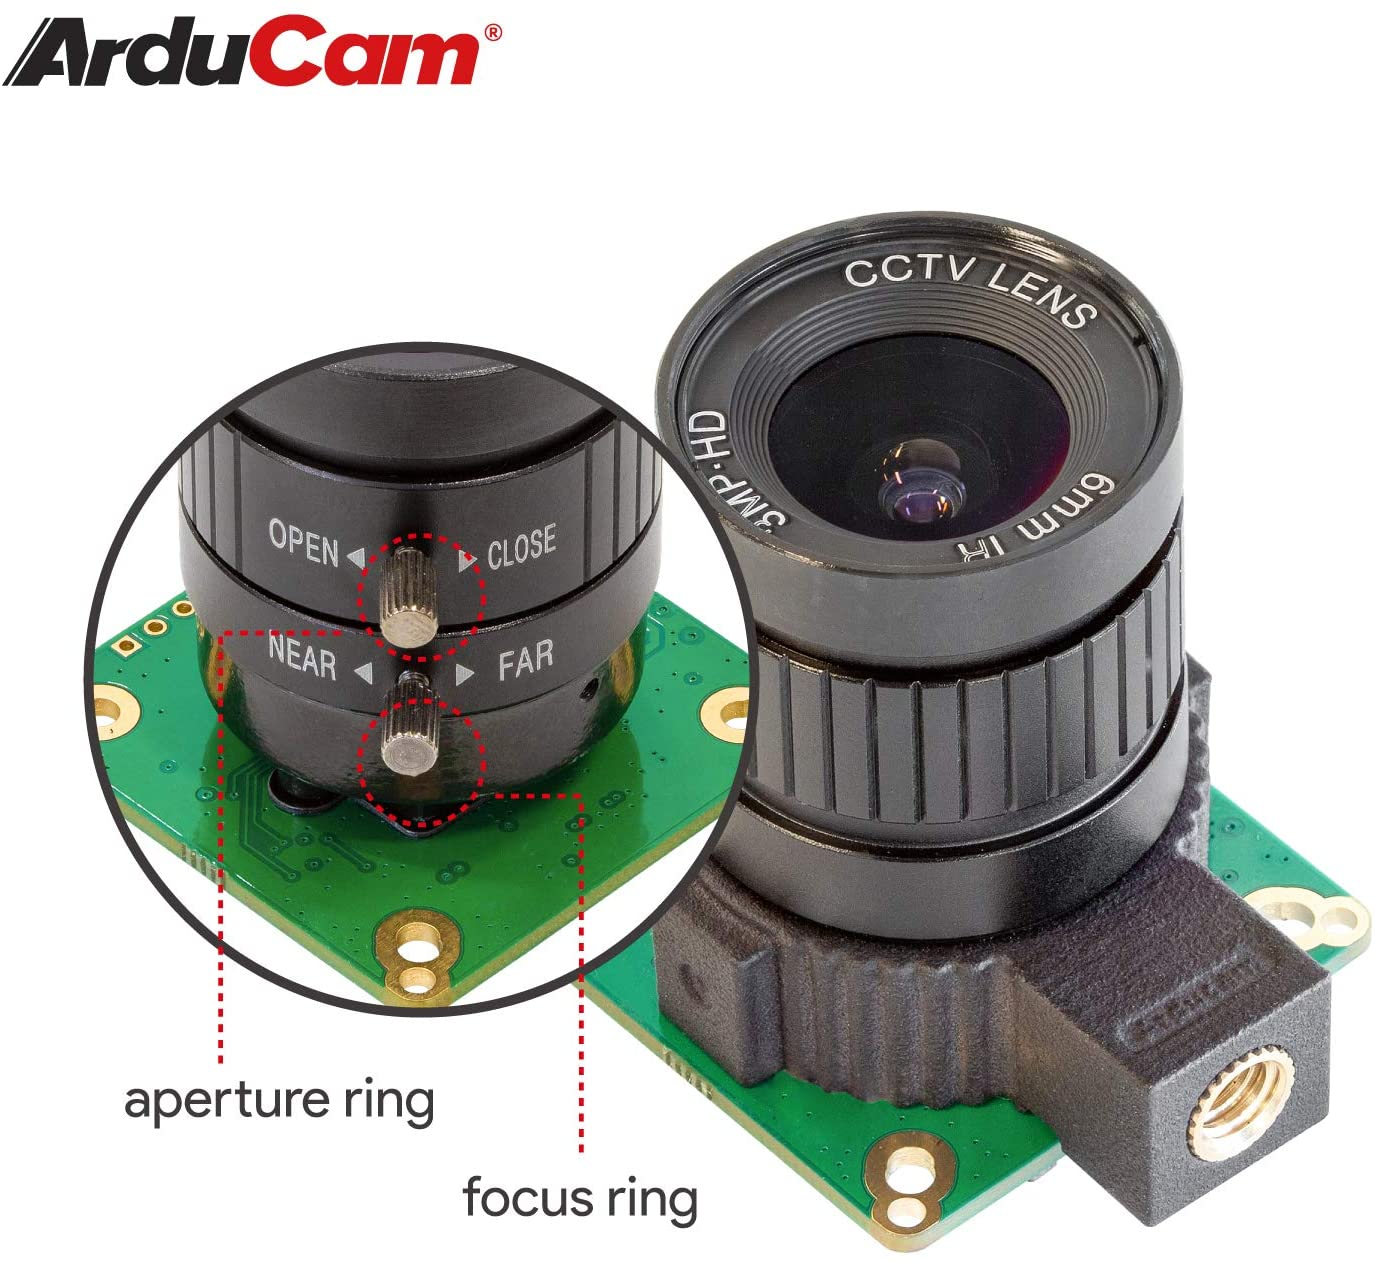
\includegraphics[scale=0.1]{CAM/imx477/imx477B9}
        
        \caption{Kamera IMX477 der Firma Arducam; \cite{Arducam:2021}}
    \end{center}    
\end{figure}

International products have separate terms, are sold from abroad and may differ from local products, including fit, age ratings, and language of product, labeling or instructions



Arducam 12,3 MP IMX477 HQ Kamera-Modul mit 6 mm CS Objektiv und Tipod-Halterung für Nvidia Jetson Nano/Xavier NX und Raspberry Pi Computermodul

\url{https://www.amazon.de/Arducam-Kamera-Modul-Tipod-Halterung-Raspberry-Computermodul/dp/B08SC2QY1B/ref=pd_sbs_3/261-1564509-7527066?pd_rd_w=Bodcr&pf_rd_p=a0a2bb41-2b9d-47ea-9dff-8a3ade3a13d6&pf_rd_r=2W868QDFVHRJCGGFVZ9Q&pd_rd_r=0f94f9d1-3f4c-47c5-a17f-4dc798a15aaa&pd_rd_wg=TBqO1&pd_rd_i=B08SC2QY1B&psc=1}



    
\section{What are the Jetson Native Cameras}

Native Jetson CameraThe native cameras are the camera modules that officially supported by the Jetson hardware with the driver and ISP support. At the moment, two camera modules IMX219 and IMX477 are natively supported, they can cover most of the use-cases.

\section{What is the Advantage on Jetson Native Cameras}

If you are new to Jetson and want to use the camera with the existing on-line opensource code that uses native camera commands like nvgstcapture/nvarguscamera, or nvargus API, etc.


\url{https://www.arducam.com/docs/camera-for-jetson-nano/native-jetson-cameras-imx219-imx477/imx477/}

\url{https://www.arducam.com/docs/camera-for-jetson-nano/native-jetson-cameras-imx219-imx477/imx477-ir-cut-camera/}

\begin{code}

\begin{lstlisting}
# MIT License
# Copyright (c) 2019 JetsonHacks
# See license
# Using a CSI camera (such as the Raspberry Pi Version 2) connected to a
# NVIDIA Jetson Nano Developer Kit using OpenCV
# Drivers for the camera and OpenCV are included in the base image

import cv2

# gstreamer_pipeline returns a GStreamer pipeline for capturing from the CSI camera
# Defaults to 1280x720 @ 60fps
# Flip the image by setting the flip_method (most common values: 0 and 2)
# display_width and display_height determine the size of the window on the screen


def gstreamer_pipeline(
    capture_width=1280,
    capture_height=720,
    display_width=1280,
    display_height=720,
    framerate=60,
    flip_method=0,
):
    return (
        "nvarguscamerasrc ! "
        "video/x-raw(memory:NVMM), "
        "width=(int)%d, height=(int)%d, "
        "format=(string)NV12, framerate=(fraction)%d/1 ! "
        "nvvidconv flip-method=%d ! "
        "video/x-raw, width=(int)%d, height=(int)%d, format=(string)BGRx ! "
        "videoconvert ! "
        "video/x-raw, format=(string)BGR ! appsink"
        % (
            capture_width,
            capture_height,
            framerate,
            flip_method,
            display_width,
            display_height,
        )
    )


def show_camera():
    # To flip the image, modify the flip_method parameter (0 and 2 are the most common)
    print(gstreamer_pipeline(flip_method=0))
    cap = cv2.VideoCapture(gstreamer_pipeline(flip_method=0), cv2.CAP_GSTREAMER)
    if cap.isOpened():
        window_handle = cv2.namedWindow("CSI Camera", cv2.WINDOW_AUTOSIZE)
        # Window
        while cv2.getWindowProperty("CSI Camera", 0) >= 0:
            ret_val, img = cap.read()
            cv2.imshow("CSI Camera", img)
            # This also acts as
            keyCode = cv2.waitKey(30) & 0xFF
            # Stop the program on the ESC key
            if keyCode == 27:
                break
       cap.release()
       cv2.destroyAllWindows()
    else:
        print("Unable to open camera")


if __name__ == "__main__":
    show_camera()
\end{lstlisting}

  \caption{Beispielprogramm für CAM imx477; Quelle: \url{https://www.arducam.com/docs/camera-for-jetson-nano/native-jetson-cameras-imx219-imx477/python-example/}}
\end{code}


\begin{itemize}
  \item \url{https://github.com/JetsonHacksNano/CSI-Camera/blob/master/simple_camera.py}
  \item \url{https://www.arducam.com/docs/camera-for-jetson-nano/native-jetson-cameras-imx219-imx477/imx477-troubleshoot/}
  \item \url{https://www.arducam.com/sony/imx477/}
  \item \url{https://www.uctronics.com/camera-modules/camera-for-raspberry-pi/high-quality-camera-raspberry-pi-12mp-imx477.html}
  \item \url{https://www.arducam.com/sony/imx477/}
\end{itemize}

